\documentclass[a4paper]{scrartcl}
\usepackage[T1]{fontenc}
\usepackage{iftex}
\ifpdftex
    \usepackage[T1]{fontenc}
    \usepackage[utf8]{inputenc}
\else
    \usepackage{fontspec}
\fi
\usepackage[
    hidelinks=false,
    colorlinks=true,
    linkcolor=cyan!70!black,
    filecolor=magenta,      
    urlcolor=cyan,
]{hyperref}
\usepackage{csquotes}
\usepackage{amsmath}
\usepackage{amsfonts}
\usepackage{amsthm}
\usepackage[french]{babel}
\usepackage[
    %style=alphabetic,
    backend=biber,
    natbib=true,
    url=false,
    eprint=true,
    sorting=none,
    defernumbers=true,
    giveninits=true,
    %maxalphanames=2,
    %minalphanames=0,
    maxcitenames=3,
    maxbibnames=3,
    doi=true,
]{biblatex}
\usepackage{fontawesome}
\usepackage[dvipsnames]{xcolor}
\usepackage{graphicx}
\usepackage{listings}
\usepackage[margin=1.5cm]{geometry}
\usepackage{lmodern}    % Police Latin Computer modern
%\usepackage{tgschola}  % Police TeX Gyre Schola
%\usepackage{mathptmx}  % Police Times

\lstdefinestyle{mystyleII}{
    backgroundcolor={},
    commentstyle=\color{black!50},
    keywordstyle=\color{green!50!black},
    numberstyle=\tiny\color{black!50},
    stringstyle=\color{purple},
    basicstyle=\ttfamily\footnotesize,
    breakatwhitespace=false,
    breaklines=true,
    captionpos=b,
    keepspaces=true,
    %numbers=left,
    %numbersep=10pt,
    %linewidth=.5\textwidth,
    frame=tb,
    framerule=0.1pt,
    framexleftmargin=0pt,
    framextopmargin=0pt,
    showspaces=false,
    showstringspaces=false,
    showtabs=false,
    tabsize=2,
    aboveskip=15pt,
    belowskip=15pt,
    %resetmargins=true
}
\lstset{style=mystyleII}
\renewcommand\lstlistingname{\textsc{Codes}}
\renewcommand\lstlistlistingname{\textsc{Codes}}

\addbibresource{references.bib}

\title{MA0922 - TP3 : FORTRAN par la pratique\\ \large Matrices creuses CSR et méthode de Jacobi}
\author{Josaphat ADDA \href{mailto:josaphat.adda@etudiant.univ-reims.fr}{\faEnvelopeO}}
\date{\today}

\begin{document}
\maketitle
\tableofcontents

\section{Problème, format CSR et méthode de Jacobi}

\subsection{Le problème}

On considère la matrice tridiagonale $A\in\mathbb{R}^{n\times n}$ de diagonales constantes $a_1$ (sous-diagonale), 
$a_2$ (diagonale) et $a_3$ (sur-diagonale), et le second membre constant $b=(a_4,\dots,a_4)^\top$. La ligne $i$ du système s'écrit
\[
a_1x_{i-1}+a_2x_i+a_3x_{i+1}=a_4,
\]
les termes $x_0$ et $x_{n+1}$ n'existant pas (première et dernière lignes tronquées).

\subsection{Stockage CSR}

Le format CSR utilise trois tableaux unidimensionnels :
\begin{itemize}
\item \lstinline{val} : les valeurs non nulles, rangées ligne par ligne ;
\item \lstinline{icol} : l'indice de colonne de chaque valeur de \lstinline{val} ;
\item \lstinline{nnz} : le nombre de valeurs non nulles cumulées par ligne, en commençant par $0$.
\end{itemize}
Les valeurs non nulles de la ligne $i$ sont aux positions \lstinline{nnz(i)+1} à \lstinline{nnz(i+1)}. 
Une tridiagonale a $n$ éléments sur la diagonale et $n-1$ sur chacune des deux autres, soit $3n-2$ valeurs non nulles : 
\lstinline{val} et \lstinline{icol} ont $3n-2$ éléments, et \lstinline{nnz} en a $n+1$ puisqu'il commence par $0$. 
Pour $n=4$, on obtient $\texttt{nnz}=(0,2,5,8,10)$.

\subsection{La méthode de Jacobi}

Soit $D$ la matrice formée de la diagonale de $A$. À partir de $x^{(0)}=0$, on calcule à chaque itération le résidu
 $r^{(k)}=b-Ax^{(k)}$. Si $\|r^{(k)}\|_2<\varepsilon$, alors $x^{(k)}$ est la solution et l'algorithme s'arrête. Sinon
\[
x^{(k+1)}=x^{(k)}+D^{-1}r^{(k)}.
\]
Le pseudo-code est le suivant.
\begin{lstlisting}[language={}]
Entrees : A, b, kmax, epsilon
x <- 0 ; d <- diag(A)
Pour k = 1 a kmax :
    r <- b - A*x
    Si ||r||_2 < epsilon : converge <- vrai ; sortir
    x <- x + r / d
Fin pour
Si non converge : afficher "kmax atteint sans convergence"
\end{lstlisting}

\subsection{Convergence}

L'itération s'écrit $x^{(k+1)}=Bx^{(k)}+D^{-1}b$ avec $B=I-D^{-1}A$. Elle converge pour tout $x^{(0)}$ 
si et seulement si le rayon spectral $\rho(B)$ est strictement inférieur à $1$. Si $A$ est à diagonale strictement dominante,
 c'est-à-dire ici $|a_2|>|a_1|+|a_3|$, alors $\rho(B)<1$ : la condition est suffisante, pas nécessaire. 
 Pour une matrice tridiagonale de Toeplitz, les valeurs propres de $B$ sont connues et
\begin{equation}
\rho(B)=\frac{2\sqrt{a_1a_3}}{|a_2|}\cos\Big(\frac{\pi}{n+1}\Big).
\label{eq:rho}
\end{equation}
Cette formule permet de prévoir le comportement de l'algorithme avant de le lancer. Plus $\rho$ est proche de $0$,
plus la convergence est rapide ; si $\rho>1$, le résidu croît comme $\rho^k$.

\subsection{Itératif ou direct ?}

Pour un grand système creux, une méthode itérative a plusieurs avantages sur une méthode directe de type factorisation LU :
\begin{itemize}
\item \textbf{Mémoire} : seule $A$ est stockée, en $O(\text{nnz})$ ; une factorisation crée du remplissage (\textit{fill-in}) et demande beaucoup plus de place.
\item \textbf{Coût} : une itération est un produit matrice-vecteur creux, en $O(\text{nnz})$.
\item \textbf{Précision modulable} : on s'arrête dès que le résidu est assez petit.
\item \textbf{Parallélisation} : le produit matrice-vecteur se parallélise facilement.
\end{itemize}

\section{Implémentation en Fortran}

Le code est réparti en trois fichiers : \lstinline{matutils.f90} (module de matrices creuses), \lstinline{linearsolver.f90} (module du solveur) 
et \lstinline{verifications.f90} (programme principal).

\subsection{Le type \lstinline{MatrixSparse}}

\begin{lstlisting}[language=Fortran]
type MatrixSparse
    integer :: n = 0                  ! dimension de A (A est n x n)
    real(8), allocatable :: val(:)    ! valeurs non nulles
    integer, allocatable :: nnz(:)    ! pointeurs de lignes, taille n+1
    integer, allocatable :: icol(:)   ! indices de colonne
end type MatrixSparse
\end{lstlisting}
Le champ \lstinline{n} permet à la matrice de porter sa propre taille : une procédure qui reçoit \lstinline{A} 
n'a pas besoin d'un argument supplémentaire, ce qui évite les incohérences. Il ne se déduit pas de \lstinline{val} 
ou \lstinline{icol}, qui ne contiennent que les non-nuls. L'initialisation \lstinline{n = 0} signifie qu'une matrice 
fraîchement déclarée est vide. Le symbole \lstinline{%} sert à accéder à un champ : \lstinline{A%n}, \lstinline{A%val}, \lstinline{C%nnz}.

\subsection{Construction, trace et norme}

La fonction \lstinline{tridiag(n,a1,a2,a3)} alloue les trois tableaux (tailles $3n-2$, $n+1$, $3n-2$) 
puis les remplit ligne par ligne. Ses arguments sont déclarés \lstinline{intent(in)} : 
ils sont lus mais jamais modifiés, et le compilateur refuse toute écriture par erreur, 
ce qui évite de modifier à son insu une variable de l'appelant (Fortran passe les arguments par référence).

La trace somme les éléments dont l'indice de colonne est égal à celui de la ligne. 
La norme infinie est le maximum sur les lignes de la somme des valeurs absolues :
\[
\|A\|_\infty=\max_i\sum_j|a_{ij}|.
\]
Pour notre tridiagonale, $\operatorname{tr}(A)=na_2$ et $\|A\|_\infty=|a_1|+|a_2|+|a_3|$ si les trois diagonales sont de même signe.

\subsection{Surcharge de l'opérateur \lstinline{*}}

Surcharger un opérateur, c'est indiquer au compilateur quelle fonction appeler lorsqu'il est appliqué à 
des types qu'il ne connaît pas nativement :
\begin{lstlisting}[language=Fortran]
interface operator(*)
    module procedure matvec, matmat
end interface operator(*)
\end{lstlisting}
Le choix de la fonction se fait d'après les types des opérandes : \lstinline{A*x} (matrice et vecteur) appelle 
\lstinline{matvec}, \lstinline{A*B} (deux matrices) appelle \lstinline{matmat}, et la multiplication usuelle
des réels n'est pas modifiée. Les fonctions associées doivent avoir deux arguments \lstinline{intent(in)},
et l'ordre compte : \lstinline{x*A} n'est pas défini. Cette surcharge ne change pas le calcul, mais le rend lisible : 
le résidu de Jacobi s'écrit \lstinline{r = b - A*x}.

\subsection{Produit matrice-vecteur et matrice-matrice}

Le produit matrice-vecteur parcourt les non-nuls ligne par ligne, avec un coût en $O(\text{nnz})$ :
\begin{lstlisting}[language=Fortran]
do i = 1,A%n
    do j = A%nnz(i)+1,A%nnz(i+1)
        y(i) = y(i) + A%val(j)*x(A%icol(j))
    end do
end do
\end{lstlisting}

Le produit creux $\times$ dense est simple, car le résultat est dense et sa taille est connue. 
Le produit creux $\times$ creux est plus délicat, pour plusieurs raisons :
\begin{itemize}
\item la structure de $C=AB$ (nombre et position des non-nuls) est inconnue à l'avance : on alloue des tableaux de taille \lstinline{maxnnzC}, un majorant calculé par une première boucle, puis on recopie aux tailles exactes ;
\item plusieurs termes $A_{ik}B_{kj}$ tombent dans la même case $C_{ij}$ : on les additionne dans un tableau de travail \lstinline{w}, et un tableau logique \lstinline{used} indique si une colonne a déjà été rencontrée dans la ligne courante. Tester \lstinline{w(j) /= 0} serait faux, car une somme peut valoir exactement $0$ par annulation ;
\item le produit est en général moins creux que ses facteurs (\textit{fill-in}) : le carré d'une tridiagonale est pentadiagonal ;
\item les accès sont indirects, donc moins favorables au cache, et les colonnes de $C$ ne sont pas triées.
\end{itemize}
Après chaque ligne, seules les colonnes touchées sont remises à zéro dans \lstinline{w} et \lstinline{used}, 
de sorte que le coût d'une ligne reste proportionnel à son nombre de non-nuls. Le tableau des pointeurs de lignes est 
transféré dans \lstinline{C%nnz} par \lstinline{move_alloc}, sans se répéter. 

\subsection{Le solveur et le programme de vérification}

La routine \lstinline{jacobi(A,b,x,kmax,epsilon,converge,iter)} extrait d'abord la diagonale, puis itère comme dans le 
pseudo-code, avec la norme euclidienne calculée par \lstinline{sqrt(dot_product(r,r))}. Elle renvoie en plus un booléen
\lstinline{converge} et le nombre d'itérations \lstinline{iter}, ce qui permet d'indiquer si $k_{\max}$ a été atteint.

Le programme \lstinline{verifications} lit $n$, $(a_1,a_2,a_3,a_4)$, $k_{\max}$ et $\varepsilon$ dans le fichier
\lstinline{lp.dat}, alloue dynamiquement $b$ et $x$, affiche la trace et la norme, résout avec \lstinline{jacobi} 
et écrit la solution dans \lstinline{res.dat}. Il teste la dominance diagonale après la lecture et affiche un avertissement 
si $|a_2|\le|a_1|+|a_3|$. Il vérifie aussi, avec \lstinline{inquire}, que \lstinline{lp.dat} existe, ce qui remplace le 
plantage avec \textit{backtrace} par un message clair. Le fichier \lstinline{lp.dat} a la forme suivante :
\begin{lstlisting}[language={}]
100
1.0 4.0 2.0 1.0
1000 1.0e-7
\end{lstlisting}
La compilation se fait avec \lstinline{gfortran -Wall -o verif matutils.f90 linearsolver.f90 verifications.f90}.
\begin{lstlisting}[language={}]
     trace =   400.00000000000000        norme_inf =   7.0000000000000000     
 Convergence en          65 iterations
\end{lstlisting}
\section{Vérifications}

\subsection{Résolution à la main pour $n=2,3,4$}

On prend $(a_1,a_2,a_3,a_4)=(1,2,3,4)$. Pour $n=4$, le système est
\[
2x_1+3x_2=4,\quad x_1+2x_2+3x_3=4,\quad x_2+2x_3+3x_4=4,\quad x_3+2x_4=4.
\]
La dernière équation donne $x_3=4-2x_4$, la troisième donne $x_2=x_4-4$, la première donne $x_1=(16-3x_4)/2$, 
et la deuxième conduit à $12-5{,}5\,x_4=4$, donc $x_4=16/11$. Les solutions exactes sont :
\begin{table}[!ht]
\centering
\begin{tabular}{|c|l|}
\hline
$n$ & Solution exacte \\ \hline
2 & $x=(-4,\;4)$ \\ \hline
3 & $x=(-4,\;4,\;0)$ \\ \hline
4 & $x=\frac{1}{11}(64,\;-28,\;12,\;16)\approx(5{,}818;\,-2{,}545;\,1{,}091;\,1{,}455)$ \\ \hline
\end{tabular}
\caption{Solutions exactes à la main pour $(a_1,a_2,a_3,a_4)=(1,2,3,4)$.}
\label{tbl:main}
\end{table}

Cette matrice n'est pas à diagonale strictement dominante ($2<1+3$), donc la convergence de Jacobi n'est pas garantie. 
La formule~\eqref{eq:rho} donne le comportement attendu (Table~\ref{tbl:n234}).
\begin{table}[!ht]
\centering
\begin{tabular}{|c|c|l|l|}
\hline
$n$ & $\rho$ & Prévision & Résultat de \texttt{jacobi} ($k_{\max}=1000$, $\varepsilon=10^{-7}$) \\ \hline
2 & $0{,}87$ & converge & convergence en $127$ itérations, $x\approx(-4;\,4)$ \\ \hline
3 & $1{,}22$ & diverge & $k_{\max}$ atteint, résidu $\sim10^{88}$ \\ \hline
4 & $1{,}40$ & diverge & $k_{\max}$ atteint, résidu $\sim10^{147}$ \\ \hline
\end{tabular}
\caption{Comportement de Jacobi pour $n=2,3,4$.}
\label{tbl:n234}
\end{table}
Pour $n=2$, l'algorithme converge bien que la matrice ne soit pas dominante, ce qui illustre que la dominance est 
une condition suffisante et non nécessaire. Les ordres de grandeur des résidus pour $n=3$ et $n=4$ sont ceux de 
$\rho^{1000}$ ($1{,}22^{1000}\approx10^{88}$ et $1{,}40^{1000}\approx10^{147}$).

\subsection{Cas $n=100$, $k_{\max}=1000$, $\varepsilon=10^{-7}$}

On compare plusieurs jeux $(a_1,a_2,a_3,a_4)$ (Table~\ref{tbl:cas}). La trace vaut $na_2$ et la norme infinie 
$a_1+a_2+a_3$ dans tous les cas (valeurs positives).
\begin{table}[!ht]
\centering
\small
\begin{tabular}{|c|c|c|c|c|c|l|}
\hline
$(a_1,a_2,a_3,a_4)$ & trace & norme & dominante & $\rho$ & itér. & résultat \\ \hline
$(1,2,3,4)$ & 200 & 6 & non & $1{,}73$ & 1000 & diverge (résidu \texttt{Infinity}) \\ \hline
$(1,4,2,1)$ & 400 & 7 & oui & $0{,}71$ & 65 & converge \\ \hline
$(1,6,1,1)$ & 600 & 8 & oui & $0{,}33$ & 18 & converge \\ \hline
$(1,3,1,1)$ & 300 & 5 & oui & $0{,}67$ & 47 & converge \\ \hline
$(2,4,2,1)$ & 400 & 8 & non (égalité) & $0{,}9995$ & 1000 & non convergé (résidu $\approx5{,}6$) \\ \hline
$(3,4,3,1)$ & 400 & 10 & non & $1{,}50$ & 1000 & diverge (résidu \texttt{Infinity}) \\ \hline
\end{tabular}
\caption{Comparaison de plusieurs jeux de diagonales pour $n=100$.}
\label{tbl:cas}
\end{table}

\textbf{Cas non dominant $(1,2,3,4)$.} Avec $\rho\approx1{,}73$, le résidu croît comme $1{,}73^k$. 
Les composantes du résidu dépassent $10^{154}$ vers l'itération $650$ ; leur carré, calculé dans \lstinline{dot_product}, 
dépasse alors le maximum des réels en double précision ($\approx1{,}8\cdot10^{308}$), et la norme devient \lstinline{Infinity}. 
Le test \lstinline{Infinity < epsilon} est faux, donc la boucle va jusqu'à $k_{\max}$ et le programme indique l'absence de 
convergence. L'avertissement de dominance est affiché après la lecture de \lstinline{lp.dat}.

\textbf{Cas dominants.} Le nombre d'itérations dépend de $\rho$ : plus la dominance est forte, plus $\rho$ est petit et moins
il faut d'itérations ($18$ pour $a_2=6$, $47$ pour $a_2=3$). Pour $(1,4,2)$, la prévision asymptotique $\ln(10^8)/\ln(1/\rho)\approx53$ 
sous-estime les $65$ itérations observées. L'explication probable est que la matrice n'est pas symétrique ($a_1\ne a_3$) : 
la matrice d'itération est alors non normale, et le résidu décroît moins vite que $\rho^k$ au début.

\textbf{Cas limite $(2,4,2)$.} On a $a_2=a_1+a_3$ : la dominance n'est pas stricte, $\rho=0{,}9995$ est très proche de $1$, 
et le résidu est encore de $5{,}6$ après $1000$ itérations. Un message d'avertissement est bien affiché, et il ne s'agit pas 
d'une divergence mais d'une convergence extrêmement lente.

\textbf{Allure de la solution.} La Figure~\ref{fig:sol} montre la solution pour $(1,4,2,1)$, enregistrée dans \lstinline{res.dat}.
\begin{figure}[!ht]
\centering
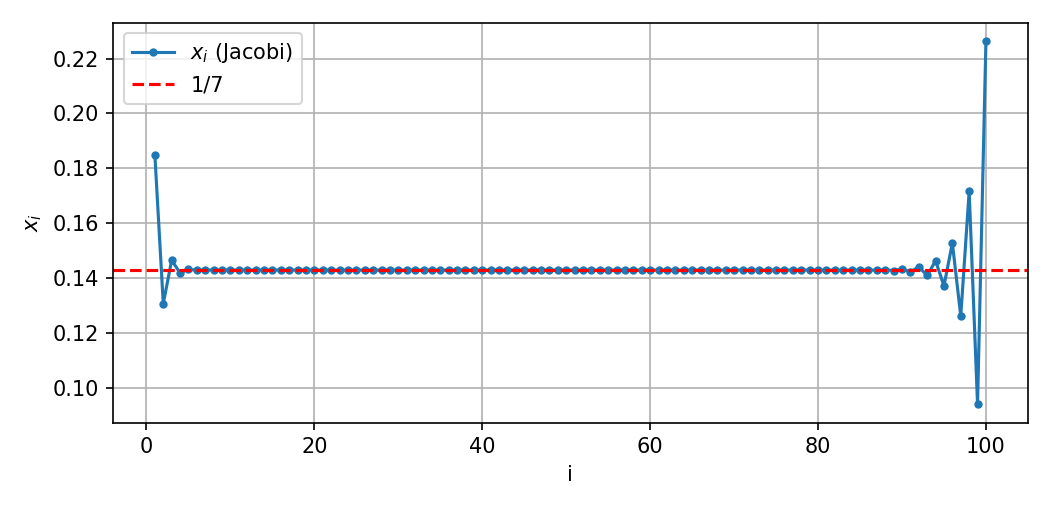
\includegraphics[width=0.85\textwidth]{img/solution.png}
\caption{Solution de $Ax=b$ pour $(a_1,a_2,a_3,a_4)=(1,4,2,1)$ et $n=100$ ; la droite en pointillés est $1/7$.}
\label{fig:sol}
\end{figure}
Loin des bords, la solution est constante et vaut $a_4/(a_1+a_2+a_3)=1/7\approx0{,}142857$, valeur qui vérifie l'équation 
intérieure $x+4x+2x=1$. Aux bords, les équations sont tronquées et la solution s'en écarte par une perturbation oscillante 
qui s'amortit en s'éloignant du bord. À gauche, les écarts à $1/7$ valent successivement $+0{,}042$, $-0{,}012$, $+0{,}0036$, 
chacun étant environ $-0{,}29$ fois le précédent, ce qui correspond à la racine de module inférieur à $1$ de $2r^2+4r+1=0$. 
À droite, la perturbation est plus marquée ($x_{100}=0{,}2265$), car c'est la sur-diagonale, de coefficient $2$, qui manque. 
On vérifie la dernière équation : $x_{99}+4x_{100}=0{,}0938+0{,}9062=1$.

\section{Expériences complémentaires}

Pour compléter les vérifications, nous avons fait varier la taille $n$, le seuil $\varepsilon$ et $k_{\max}$, 
puis testé le code sur deux exemples d'application. Chaque cas correspond à un fichier \lstinline{lp.dat} 
(les lignes sont $n$ ; $a_1\ a_2\ a_3\ a_4$ ; $k_{\max}\ \varepsilon$) lu par \lstinline{verifications}, ce qui permet de les reproduire.

\subsection{Influence de la taille $n$}

On garde $(a_1,a_2,a_3,a_4)=(1,4,2,1)$, $k_{\max}=1000$ et $\varepsilon=10^{-7}$, et on fait varier $n$ (Table~\ref{tbl:varn}).
\begin{table}[!ht]
\centering
\begin{tabular}{|r|c|c|c|c|}
\hline
$n$ & itérations & $x_1$ & $x_{n/2}$ & $x_n$ \\ \hline
10 & 48 & 0,18414 & 0,15262 & 0,22654 \\ \hline
50 & 63 & 0,18470 & 0,142857 & 0,22654 \\ \hline
100 & 65 & 0,18470 & 0,142857 & 0,22654 \\ \hline
500 & 68 & 0,18470 & 0,142857 & 0,22654 \\ \hline
1000 & 69 & 0,18470 & 0,142857 & 0,22654 \\ \hline
10000 & 74 & 0,18470 & 0,142857 & 0,22654 \\ \hline
100000 & 78 & 0,18470 & 0,142857 & 0,22654 \\ \hline
\end{tabular}
\caption{Effet de $n$ pour $(1,4,2,1)$.}
\label{tbl:varn}
\end{table}
Les valeurs de bord $x_1$ et $x_n$ ne dépendent presque pas de $n$ : la perturbation due aux bords est locale. 
La valeur au milieu vaut $1/7$ dès que $n$ est assez grand ; pour $n=10$, les perturbations venant des deux bords 
se recouvrent encore au centre ($x_5=0{,}1526$). Le nombre d'itérations augmente très lentement, d'environ $3$ à $5$ à 
chaque multiplication de $n$ par $10$ (Figure~\ref{fig:exp}, à gauche), car le rayon spectral~\eqref{eq:rho} est quasi 
constant ($0{,}71$) et seul le résidu initial $\|b\|_2=\sqrt n$ grandit.

\subsection{Influence de $\varepsilon$ et de $k_{\max}$}

Pour $n=100$ et $(1,4,2,1)$, le nombre d'itérations croît linéairement avec le nombre de chiffres demandés 
(Table~\ref{tbl:vareps}) : environ $16$ itérations de plus chaque fois que $\varepsilon$ est divisé par $100$.
\begin{table}[!ht]
\centering
\begin{tabular}{|c|c|c|}
\hline
$\varepsilon$ & itérations & résidu final \\ \hline
$10^{-3}$ & 33 & $9{,}2\cdot10^{-4}$ \\ \hline
$10^{-5}$ & 49 & $8{,}9\cdot10^{-6}$ \\ \hline
$10^{-7}$ & 65 & $8{,}6\cdot10^{-8}$ \\ \hline
$10^{-9}$ & 81 & $8{,}2\cdot10^{-10}$ \\ \hline
$10^{-12}$ & 105 & $7{,}7\cdot10^{-13}$ \\ \hline
\end{tabular}
\caption{Effet de $\varepsilon$ ($n=100$, $(1,4,2,1)$).}
\label{tbl:vareps}
\end{table}
Pour $\varepsilon=10^{-7}$, l'algorithme converge en $65$ itérations. Avec $k_{\max}=64$, il s'arrête avec un résidu de 
$1{,}1\cdot10^{-7}$, juste au-dessus du seuil, et le programme indique bien « kmax atteint SANS convergence » ; 
avec $k_{\max}=65$ ou plus, il converge. Pour $k_{\max}=10$ le résidu est encore de $0{,}73$, et pour $k_{\max}=30$ de 
$2{,}2\cdot10^{-3}$.

\subsection{Application 1 : équation de Poisson en 1D}

On cherche $u$ telle que $-u''=1$ sur $]0,1[$ avec $u(0)=u(1)=0$. Avec $h=1/(n+1)$ et $x_i=ih$, les différences 
finies donnent $(-u_{i-1}+2u_i-u_{i+1})/h^2=1$, soit un système tridiagonal avec $(a_1,a_2,a_3,a_4)=(-1,2,-1,h^2)$. 
La solution exacte $u(x)=x(1-x)/2$ est un polynôme de degré $2$, que le schéma reproduit exactement : 
l'écart entre la solution de Jacobi et $u$ ne mesure donc que l'erreur d'arrêt de l'itération. 
Ici $a_2=|a_1|+|a_3|$ : la dominance n'est pas stricte (elle l'est seulement sur la première et la dernière ligne), 
et le programme affiche l'avertissement. Jacobi converge pourtant, car la matrice est irréductible et à diagonale 
dominante, mais très lentement, car $\rho=\cos(\pi/(n+1))\to1$ (Table~\ref{tbl:poisson}).
\begin{table}[!ht]
\centering
\begin{tabular}{|c|c|c|c|c|}
\hline
$n$ & $\rho$ & itérations & $\max_i|x_i-u(x_i)|$ & itérations$/n^2$ \\ \hline
10 & 0,9595 & 469 & $5\cdot10^{-10}$ & 4,7 \\ \hline
20 & 0,9888 & 1635 & $1{,}4\cdot10^{-9}$ & 4,1 \\ \hline
40 & 0,99707 & 5906 & $3{,}8\cdot10^{-9}$ & 3,7 \\ \hline
80 & 0,99925 & 21706 & $1{,}0\cdot10^{-8}$ & 3,4 \\ \hline
160 & 0,99981 & 80356 & $2{,}9\cdot10^{-8}$ & 3,1 \\ \hline
\end{tabular}
\caption{Poisson 1D avec $\varepsilon=10^{-10}$ et $k_{\max}=200000$.}
\label{tbl:poisson}
\end{table}
Le nombre d'itérations est multiplié par environ $4$ quand $n$ double, soit une croissance en 
$n^2$ (Figure~\ref{fig:exp}, à droite). C'est cohérent avec $1-\rho\approx\pi^2/(2(n+1)^2)$ et avec 
l'estimation $k\approx 2(n+1)^2\ln(\|r^{(0)}\|/\varepsilon)/\pi^2$. Avec $k_{\max}=1000$, le programme ne converge que 
pour $n=10$ ($469$ itérations) ; dès $n=20$ ($1635$ itérations), il affiche le message d'absence de convergence. 
L'erreur finale augmente avec $n$ bien que le résidu soit le même, car $A$ devient de plus en plus mal conditionnée. 
\begin{figure}[!ht]
\centering
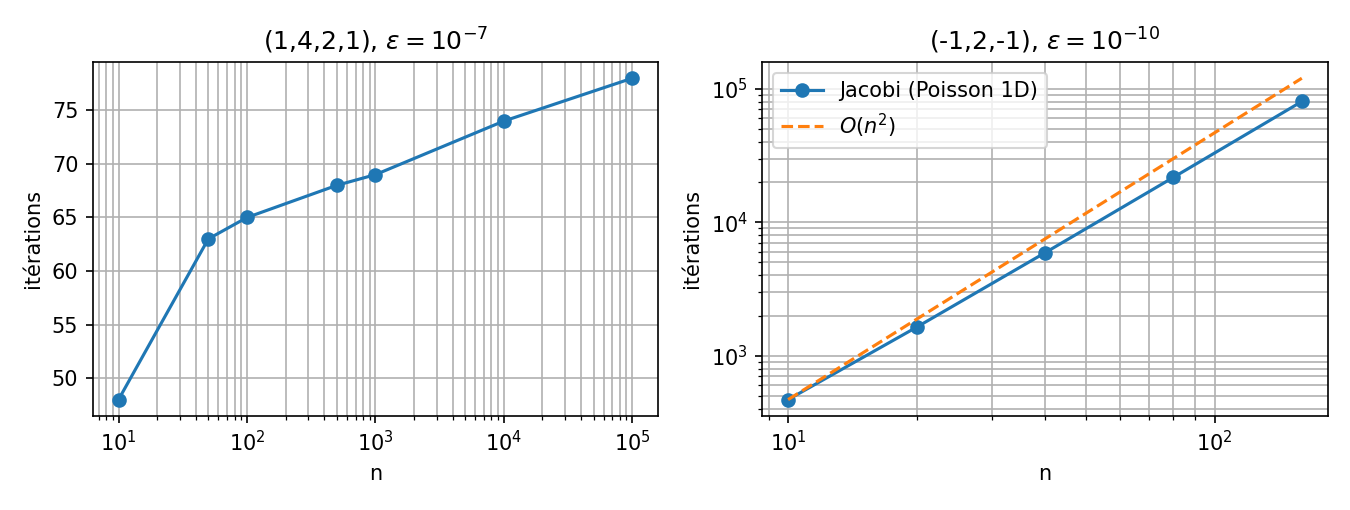
\includegraphics[width=\textwidth]{img/experiences.png}
\caption{À gauche : itérations en fonction de $n$ pour $(1,4,2,1)$. À droite : itérations en fonction de $n$ pour Poisson 1D (échelle log-log, avec une droite en $O(n^2)$).}
\label{fig:exp}
\end{figure}

\subsection{Application 2 : un pas d'Euler implicite pour l'équation de la chaleur}

Pour $u_t=u_{xx}$ sur $]0,1[$ avec $u=0$ aux bords, un pas d'Euler implicite de pas 
$\Delta t$ donne $(I+\lambda K)u^{new}=u^{old}$ avec $\lambda=\Delta t/h^2$ et 
$K=\mathrm{tridiag}(-1,2,-1)$, soit $(a_1,a_2,a_3)=(-\lambda,1+2\lambda,-\lambda)$. 
Partant de $u^{old}\equiv1$ (donc $a_4=1$) et $n=100$, la matrice est à diagonale strictement dominante pour tout 
$\lambda>0$, donc Jacobi converge toujours. 
Mais $\rho=\frac{2\lambda}{1+2\lambda}\cos\!\big(\frac{\pi}{n+1}\big)$ tend vers $1$ quand $\lambda$ 
augmente (Table~\ref{tbl:chaleur}) : plus le pas de temps est grand, plus Jacobi est lent.
\begin{table}[!ht]
\centering
\begin{tabular}{|c|c|c|}
\hline
$\lambda$ & $\rho$ & itérations ($\varepsilon=10^{-10}$) \\ \hline
0,5 & 0,50 & 38 \\ \hline
1 & 0,67 & 64 \\ \hline
5 & 0,91 & 265 \\ \hline
20 & 0,975 & 1004 \\ \hline
\end{tabular}
\caption{Euler implicite pour la chaleur ($n=100$).}
\label{tbl:chaleur}
\end{table}
Le cas $\lambda=20$ demande $1004$ itérations : avec $k_{\max}=1000$, le programme s'arrête juste avant la convergence. 
La solution vaut $1$ à l'intérieur, car la somme de chaque ligne de $A$ est $1$, et elle s'écarte de $1$ seulement 
près des bords où la condition $u=0$ agit.

\section{Benchmarks}

\subsection{Système choisi}

Le système de référence est la tridiagonale $(-1,4,-1)$ avec $b=(1,\dots,1)^\top$. Ce choix est reproductible (pas d'aléa), 
à diagonale strictement dominante ($4>1+1$, convergence garantie) et creux. 
D'après la formule~\eqref{eq:rho}, $\rho=\frac12\cos\!\big(\frac{\pi}{n+1}\big)<\frac12$ quel que soit $n$, 
de sorte que le nombre d'itérations varie peu avec la taille, ce qui isole l'effet de $n$ sur le temps. 
Le coût d'une itération est $O(\text{nnz})=O(n)$.

La procédure \lstinline{bench(n)} construit la matrice, puis mesure avec \lstinline{system_clock} le temps de 
\lstinline{jacobi} seul ($\varepsilon=10^{-8}$, $k_{\max}=10^4$).

\subsection{Interface Python avec \lstinline{f2py}}

La procédure \lstinline{bench} est exposée à Python avec \lstinline{f2py} :
\begin{lstlisting}[language={}]
python3 -m numpy.f2py -c matutils.f90 linearsolver.f90 bench.f90 -m fbench only: bench
\end{lstlisting}
Avec Python $\ge3.12$, \lstinline{f2py} utilise \lstinline{meson} comme outil de compilation, 
qu'il faut donc installer. L'option \lstinline{only: bench} est essentielle : \lstinline{f2py} 
ne sait pas convertir un type dérivé comme \lstinline{MatrixSparse} en objet Python, et sans elle il tente 
d'envelopper \lstinline{jacobi}, ce qui échoue avec l'erreur \lstinline{No C-type found ... assuming void} 
puis \lstinline{KeyError: 'void'}. Les modules \lstinline{matutils} et \lstinline{linearsolver} sont compilés 
et liés, mais pas enveloppés. L'interface avec Python passe donc par une procédure frontale à arguments simples 
(\lstinline{integer}, \lstinline{real(8)}) qui construit la matrice en interne : c'est l'intérêt de la gestion de la visibilité des modules.

Le script \lstinline{run_benchmarks.py} appelle \lstinline{fbench.bench(n)} pour $n=10^2,10^3,\dots,10^6$ 
et trace les temps avec \lstinline{matplotlib}.

\subsection{Résultats}

\begin{figure}[!ht]
\centering
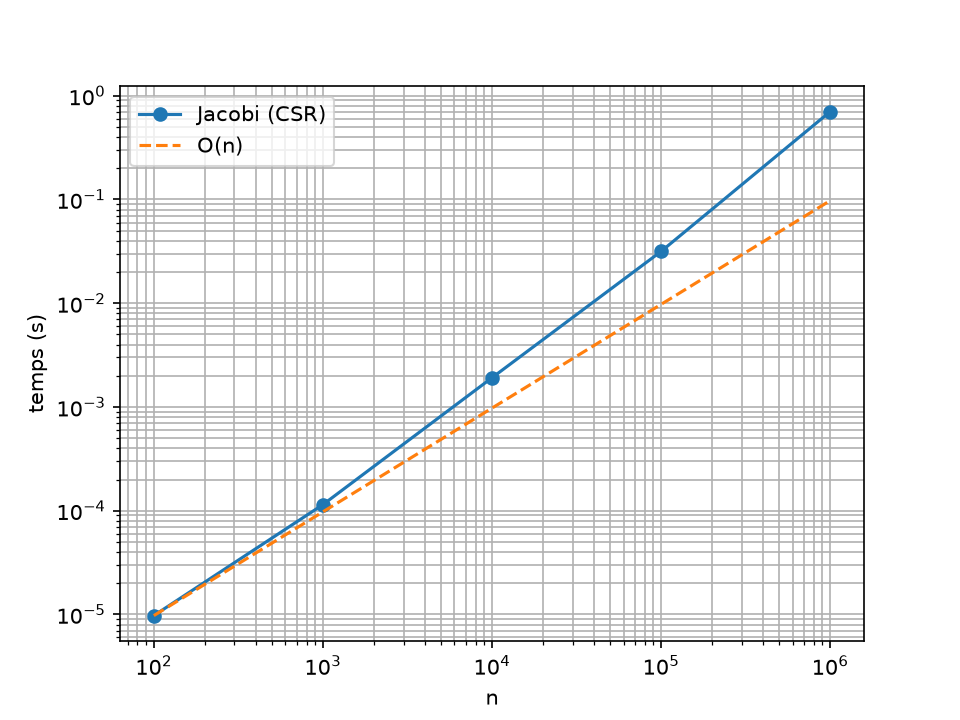
\includegraphics[width=0.75\textwidth]{img/bench.png}
\caption{Temps de résolution en fonction de $n$ (échelle logarithmique). La droite en pointillés est une loi en $O(n)$ normalisée sur le premier point.}
\label{fig:bench}
\end{figure}

La Table~\ref{tbl:bench} donne les valeurs lues sur le graphique (approximatives), 
le nombre d'itérations de Jacobi pour ce système, et le temps par itération et par inconnue.
\begin{table}[!ht]
\centering
\begin{tabular}{|c|c|c|c|c|}
\hline
$n$ & temps (s) & facteur & itérations & ns par itér. et par inconnue \\ \hline
$10^2$ & $1\cdot10^{-5}$ & -- & 31 & 3 \\ \hline
$10^3$ & $1{,}1\cdot10^{-4}$ & 12 & 33 & 4 \\ \hline
$10^4$ & $1{,}9\cdot10^{-3}$ & 17 & 35 & 5 \\ \hline
$10^5$ & $3{,}2\cdot10^{-2}$ & 17 & 36 & 9 \\ \hline
$10^6$ & $0{,}7$ & 21 & 38 & 18 \\ \hline
\end{tabular}
\caption{Temps de résolution (lus sur la Figure~\ref{fig:bench}) et itérations.}
\label{tbl:bench}
\end{table}

\subsection{Analyse}

La courbe est une droite en échelle log-log, donc le temps suit une loi de puissance en $n$. 
Entre $10^2$ et $10^3$, elle se superpose à la droite $O(n)$. Au-delà, elle s'en écarte : 
à chaque multiplication de $n$ par $10$, le temps est multiplié par $17$ à $21$ au lieu de $10$, 
soit une pente d'environ $1{,}2$ à $1{,}3$. Le comportement est donc légèrement sur-linéaire, 
et non strictement linéaire comme on pouvait l'anticiper.

Le nombre d'itérations n'explique qu'une petite partie de l'écart : il passe de $31$ à $38$ (facteur $1{,}2$), 
car le critère d'arrêt porte sur la norme euclidienne absolue du résidu, dont la valeur initiale est $\sqrt n$. 
Le reste vient du temps par itération et par inconnue, qui est multiplié par $6$ entre $n=10^2$ et $n=10^6$. 
Les causes probables, à confirmer par des mesures complémentaires, sont :
\begin{itemize}
\item les \textbf{effets de cache} : pour $n=10^6$, \lstinline{val} et \lstinline{icol} occupent environ $36$~Mo, auxquels s'ajoutent les vecteurs $x$, $r$, $d$ et $b$ ($8$~Mo chacun). L'ensemble dépasse les caches du processeur et chaque itération est limitée par la bande passante mémoire ;
\item les \textbf{tableaux temporaires} : \lstinline{r = b - A*x} crée un tableau résultat pour \lstinline{matvec} à chaque itération, ce qui augmente le trafic mémoire ;
\item la \textbf{résolution du chronomètre} : pour $n=10^2$, le temps est de l'ordre de $10~\mu$s, ce qui rend la mesure peu précise.
\end{itemize}


\end{document}
